
\cleardoublepage

\chapter{Desarrollo Hardware}
\label{makereference4}

Antes de comenzar programando la funcionalidad principal de este proyecto, tuvimos que aprender a utilizar herramientas y conceptos como los entornos de desarrollo de las placas de Nordic y de Cypress o los protocolos SPI e I2C y el propio BLE, con los que no habíamos trabajado nunca, por lo que primero realizamos una serie de pruebas para familiarizarnos y así decidir cuál de ellas elegiríamos finalmente para el proyecto.

\section{Pruebas iniciales con Cypress y Nordic}
\label{makereference4.1}

Una vez tuvimos las placas, el primer paso fue buscar códigos de ejemplo con funcionalidades parecidas a lo que íbamos a tratar en el proyecto.

\textbf{Cypress} pone a disposición de cualquier desarrollador que desee realizar pruebas un repositorio en GitHub con 100 proyectos que sirven de ejemplo para utilizar la funcionalidad BLE de sus dispositivos PSoC. Aparte han desarrollado una aplicación Android llamada \textit{CySmart} para comprobar el funcionamiento de algunos de estos ejemplos.

\textbf{mbed} dispone de un repositorio propio donde cualquier usuario puede subir proyectos para cualquier dispositivo compatible con mbed. Estos proyectos son muy sencillos de buscar e importar desde el propio compilador. ARM mbed también dispone de una app Android, ésta llamada \textit{nRF Master Control Panel}, que permite hacer algunas pruebas.

Como primera toma de contacto con las posibilidades de las placas para comunicarse físicamente con otros dispositivos realizamos un pequeño circuito consistente en una fotoresistencia conectada a un conversor analógico-digital MCP3008, capaz de convertir una entrada analógica de voltaje en un valor binario, el cual se transmitiría por el bus SPI.

Una vez creado el circuito comprobamos con un voltímetro que dejar pasar menos luz sobre la fotoresistencia disminuía la cantidad de voltaje. El rango de voltaje que pudimos comprobar fue de 0,82 V a 1,82 V con luz ambiente.

\begin{figure}[h]%t=top, b=bottom, h=here
	\centering
    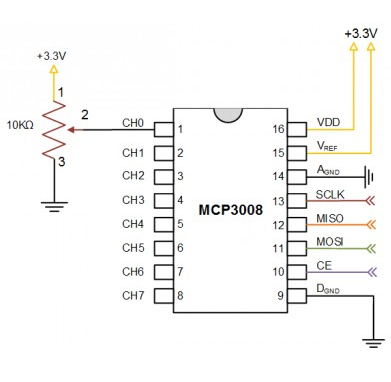
\includegraphics{figures/mcp3008_esquema.PNG} % TODO hacer que esto no quede horrible
    \caption[TODO]{TODO}
   	\label{figuraMCPEsquema}
\end{figure}

Para realizar la transferencia de datos por SPI colocamos como master la placa de desarrollo y como esclavo el circuito de la fotoresistencia. Conectamos los 4 pines correspondientes en cada placa: para la trasmisión de datos (MOSI, MISO), frecuencia de reloj (SCLK) y selección del esclavo (nSS). Ambos entornos de desarrollo ofrecen ejemplos de módulo SPI con lo que fue fácil hacer funcionar el sistema una vez conectados los pines correctos.

Para comprobar en un principio si se recibían correctamente los datos, en la placa nRF51-DK de Nordic utilizamos sus 4 LED’S verdes, apagándolos o encenciéndolos según el valor ya digitalizado que recibe. De igual forma al probarlo con PSoC BLE de Cypress interactuamos con su LED RGB, utilizando los colores verde, azul y rojo para representar los diferentes datos que recibía del circuito.

Estas primeras pruebas nos sirvieron para comprobar la correcta recepción de datos, pero el objetivo era llevarlos a una aplicación desarrollada en Android. Por tanto nuestra primera toma de contacto con el desarrollo de la aplicación Android (Figura~\ref{figuraAPPPrueba}) que hacía uso del módulo BLE fue en este momento, centrado más en la funcionalidad más que en el diseño. Esta aplicación funcional nos permitió probar conceptos como el de activar desde dentro de una app el Bluetooth del móvil, realizar un escaneo para detectar los dispositivos con Bluetooth cercanos, conectarse a éstos y enviar datos. Para verificar que funcionaba correctamente, escribimos mensajes de log  que se pueden visualizar en el entorno de desarrollo Android Studio.

\begin{figure}[h]%t=top, b=bottom, h=here
	\centering 	
    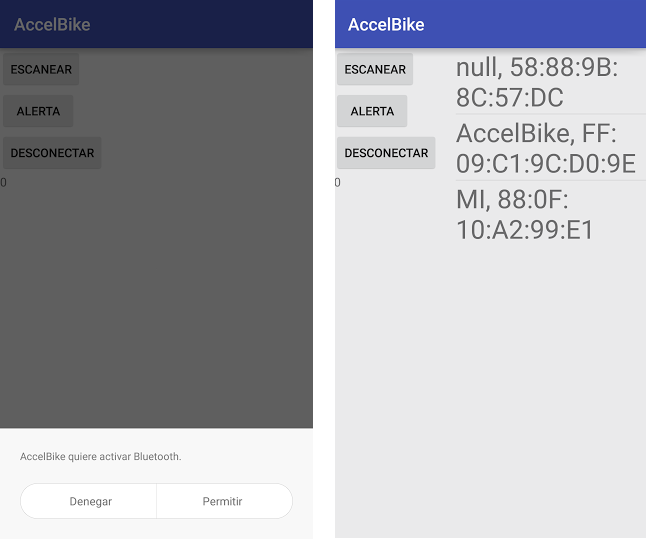
\includegraphics[width=\textwidth]{figures/app_piloto2.PNG} % TODO hacer que esto no quede horrible
   	\caption[Aplicación piloto para comprobar la conexión Bluetooth]{Aplicación piloto para comprobar la conexión Bluetooth}
   	\label{figuraAPPPrueba}
\end{figure}

El siguiente paso hacia nuestro aprendizaje fue conectar por I2C el Acelerómetro XTRINSIC-SENSE-BOARD Element14. Documentándonos desde su datasheet, conectamos los pines correctos con la placa, e iniciamos las pruebas de recepción de datos.
Nuevamente, la galería de proyectos que oferece el entorno mbed nos permitió desarrollar el código de comunicación I2C sin mucha dificultad.

% Ponemos aqui que la de Cypress no nos funcionaba y decidimos dejarla?

\section{Acerca de los entornos de desarrollo}
\label{makereference4.2}

\subsection{ARM mbed}
\label{explicacionARMmbed}

La placa de desarrollo de Nordic nRF51-DK es compatible con el entorno de desarrollo mbed. Esta herramienta, creada por la empresa ARM, pretende facilitar la programación de una gran cantidad de dispositivos IoT, eliminando la necesidad de utilizar entornos de desarrollo específicos de cada marca.\\

La interfaz del compilador mbed es \textit{online}, permitiendo, tras registrarse, acceder al entorno desde cualquier navegador en cualquier dispositivo con una conexión a Internet. El lenguaje de programación utilizado es C++, y una vez elegido a qué dispositivo va orientado el código, mbed se encarga de toda la configuración a bajo nivel, por lo que, por ejemplo, sacar una señal a través de un pin se puede realizar tan fácimente como declarar una variable \textit{DigitalOut} con su correspondiente número de pin.

Una vez tenemos un código listo, mbed permite compilarlo y descargar el archivo hexadecimal a nuestro sistema si no ha habido errores de compilación. Para cargarlo en la placa de Nordic, basta con conectar ésta al ordenador por USB, lo que la abrirá en nuestro sistema como una \textit{unidad flash} en la que podremos copiar el archivo compilado. Si ha ocurrido algún problema en la carga, o el programa cargado ha fallado por un error de ejecución, se creará en esa unidad extraíble un archivo de \textit{log} con información sobre el error.

\begin{figure}[h]%t=top, b=bottom, h=here
	\centering 	
    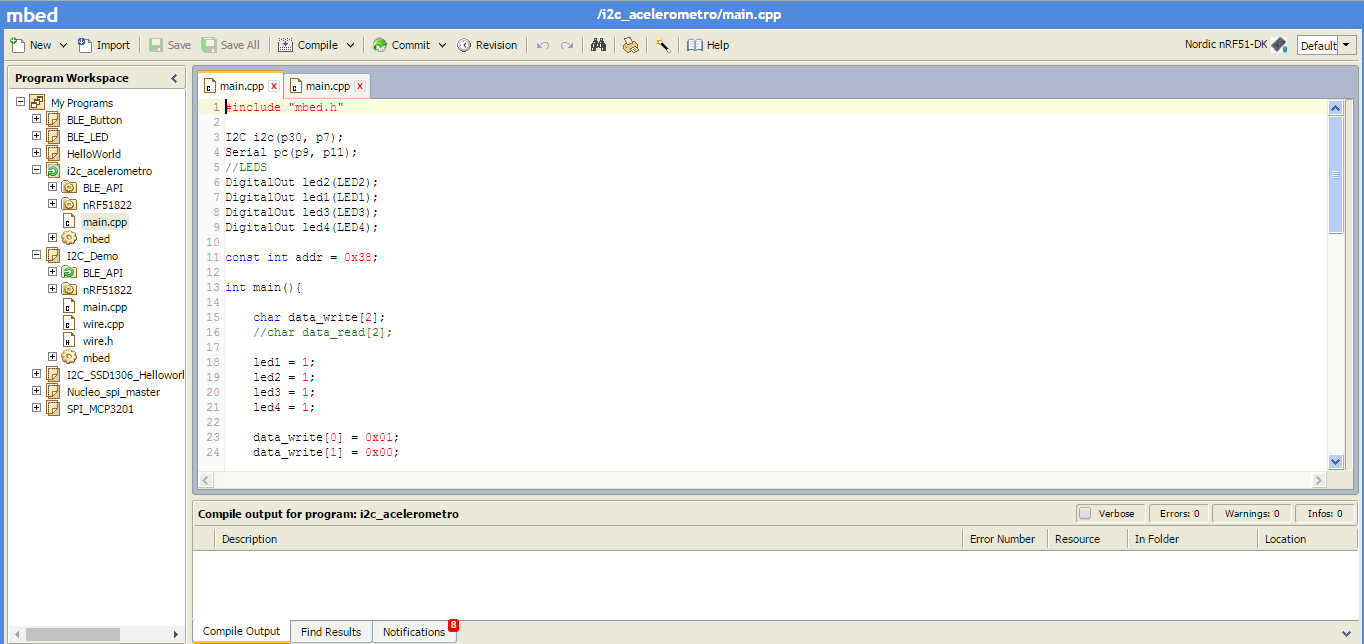
\includegraphics[width=\textwidth]{figures/mbed_compiler.PNG} % TODO hacer que esto no quede horrible
   	\caption[Entorno de desarrollo mbed]{Entorno de desarrollo mbed}
   	\label{figuraMbedCompiler}

\end{figure}

La plataforma mbed está muy orientada a la colaboración entre desarrolladores, e implementa un repositorio propio donde cualquier usuario puede subir su código y otros usuarios pueden importarlos de forma sencilla a sus proyectos. Esto se hace evidente teniendo en cuenta que en la propia interfaz se encuentra un botón \textit{Import} que abre un buscador para encontrar códigos o librerías a través de palabras clave, lo cual resultó de gran ayuda en el período de pruebas y en la fase final, como se comentaba anteriormente.\\

Como puntos negativos se puede resaltar que mbed no cuenta con ninguna herramienta de \textit{debug}, por lo que nos vimos obligados a comprobar el correcto funcionamiento de nuestros programas a través de LEDs o de \textit{printf}s, que nos permitían enviar cadenas de texto a través del puerto USB del dispositivo. También cabe destacar que, aunque el hecho de ser online supone una ventaja a la hora de trabajar desde varios sistemas, resulta un problema si no se dispone de conexión a Internet en un determinado momento.

\subsection{PSoC Creator}
\label{explicacionPSoCCreator}

\section{Motivos para quedarse con Nordic}
\label{makereference4.3}

\section{Algo más de información sobre mbed}
\label{makereference4.4}

\section{Comunicación Bluetooth}
\label{makereference4.5}

\section{Programación GPIO: XTRINSIC-SENSE-BOARD I2C, SPI}
\label{makereference4.6}

\section{SPI}
\label{makereference4.7}

\section{I2C}
\label{makereference4.8}

\subsection{Lectura de datos}
\label{makereference4.8.1}

\subsection{Filtrado}
\label{makereference4.8.2}